\chapter{Leader Election algorithms}

\begin{compactitem}
	\item many distributed algorithms require one process to act as coordinator, initiator, or otherwise perform some special role
	\item usually, it does not matter which process takes on this responsibility
	\item but one process has to be elected to take over the role 
	\item In general, election algorithms attempt to locate the process with the highest process number and designate it as coordinator
\end{compactitem}

\section{Leader election in a synchronous ring}
\begin{compactitem}
	\item Network is a graph $G$ consisting of $n$ nodes connected by unidirectional links. Use $\mod n$ for labels
	\item Synchronous time model: all processes operate in lock-step, i.e. messages are passed in synchronous rounds (needs notion of global time)
\end{compactitem}

\begin{compactitem}
\item elected node is ``leader''
\item leader election is not possible for identical processes/nodes
\item [$\rightarrow$] processes have unique id (UID)
\end{compactitem}

\subsection{LCR algorithm}
(Le Lann, Chang, Roberts)\\

\begin{compactitem}
\item unidirectional communication
\item ring size unknown
\item only leader produces output
\item algorithm compares UID
\item One or more $p_i$s can take the initiative and start an election, by sending an election message containing their id to $p_{i+1}$
\end{compactitem}

\begin{minipage}{\linewidth}
	\centering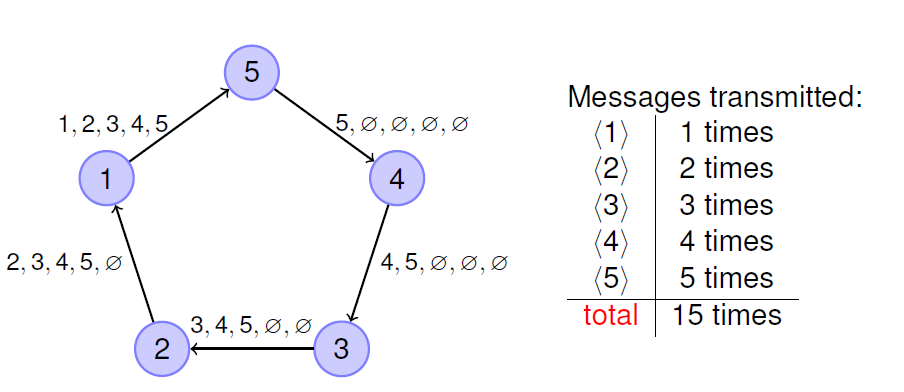
\includegraphics[width=310px]{gfx/lcr.png}
	\captionof{figure}{LCR algorithm}
	\label{img:lcr}
\end{minipage}

\subsubsection*{Algorithm (from lecture) }

\begin{lstlisting}[mathescape, language=VHDL, keywordstyle=\ttfamily]
For each node
	u = a UID, initially i's UID
	send = a UID or NULL, initially i's UID
	status $\in$ {unknown, leader} initially unknown

message generation
	send = current value of send to node i+1

state transitions
	send = NULL
	if incoming message is v (a UID) then
		v > u: 	send v
		v = u: 	status=leader
		v < u: 	do nothing
\end{lstlisting}
\ \\

\subsubsection*{Algorithm (alternative formulation)}
\begin{lstlisting}[mathescape]
upon receiving no message
	send uid_$i$ to left (clockwise)

upon receiving m from right
	if m.uid > uid$_i$:
		send m to left
	if m.uid < uid$_i$:
		discard m
	if m.uid = uid$_i$:
		leader := i
		send <terminate, i> to left 12: terminate

upon receiving <terminate, i> from right
	leader := i
	send <terminate, i> to left 
	terminate
\end{lstlisting}

\subsubsection*{Algorithm: Informal}

\begin{compactitem}
	\item One or more $p_i$'s can take the initiative and start an election, by sending an election message containing their id to $p_{i+1}$
	\item When a process receives a UID, it compares this one to its own:
	\begin{compactitem}
		\item If the incoming UID is greater, then it passes this UID to the next process.
		\item If the incoming UID is smaller, then it discards it
		\item If it is equal, then the process declares itself the leader.
	\end{compactitem}
	\item (the received uid is not saved, even if it is greater than the own uid, i.e. received uids are always compared against the own uid)
\end{compactitem}


\subsubsection*{Correctness}
Let max index of process with $max(UID)$ let $u_{max}$ is its UID\\
Show:\\
\begin{compactitem}
\item[(i)] process max outputs ``leader'' after $n$ rounds
\item[(ii)] no other process does the same
\end{compactitem}

We clarify:\\
\begin{compactitem}
\item[(iii)] After $n$ rounds status$_{max}$=leader
\end{compactitem}
and\\
\begin{compactitem}
\item[(iv)] For $0\leq r\leq n-1$ after $r$ rounds\\
	$send_{max}=u_{max}$
\end{compactitem}
find UID at distance $r$ from $i_{max}$ as it has to go once around.\\

Show $(iv)$ for all r: Induction\\
then (iii)\\

\subsubsection*{Complexity}
\begin{compactitem}
\item time complexity is $n$ rounds
\item communication complexity $\mathcal{O}(n^2)$
\item not very expensive in time, but many messages

\end{compactitem}

\subsection{Algorithm of Hirschberg and Sinclair (HS-Alg)}
\begin{compactitem}
	\item election needs to be started at every node, e.g. by a broadcast to all nodes to start leader election
\end{compactitem}

\subsubsection*{Algorithm (informal)}
\begin{compactitem}
	\item ring is bidirectional
	\item each process $p_i$ operates in phases
	\item in each phase r, pi sends out “tokens” containing uidi in both direction
	\item Tokens are intended to travel distance $2^r$ and return to $p_i$
	\item however, tokens may not make it back
	\item Token continues outbound only if greater than tokens on path
	\item Otherwise discarded
	\item All processes always forward tokens moving inbound
	\item if $p_i$ receives its own token while it is going outbound, $p_i$ is the leader
\end{compactitem}

\subsubsection{Algorithm}
\begin{lstlisting}[mathescape, language=VHDL]
each process has states with components
	u, UID: initially i's UID
	send+ containing NULL or (UID, flag{in, out}, hopcount): initially (i's UID, out, 1)
	send- as send+
	status $\in${unknown, leader} initailly unknown 
	phase $\in N$: initially 0

message generation
	send current send+ to process i+1
	send current send- to process i-1

state transitions
	send+=NULL
	send-=NULL
	if message from (i-1) is (v, out, h) then
		v>u $\land$ h>1: send+ = (v,out,h-1)
		v>u $\land$ h=1: send- = (v,in,1)
		v=u status = leader
	if message from i+1 is (v, out, h) then
		v>u $\land$ h>1: send- = (v,out, h-1)
		v>u $\land$ h=1: send+ = (v,in,1)
		v=u status=leader
	if message from i-1 is (v,in,1) $\land v\neq u$ then
		send+=(v,in,1)
	if message from i+1 is (v,in,1) $\land v\neq u$ then
		send-=(v,in,1)
	if both messages from i-1 and i+1 are (u,in,1) then
		phase++
		send+=(u,out, $2^{phase}$)
		send-=(u,out, $2^{phase}$)
\end{lstlisting}
\ \\

\subsubsection{Complexity}
\begin{compactitem}
	\item \textbf{Communication complexity}
	\begin{compactitem}
		\item Total number of phases is at most $8n(1+\lceil\log(n)\rceil)$
		\item the total number of messages is at most in $(1+\lceil(\log(n))\rceil$	
		\item $\Rightarrow \mathcal{O}(n\log n)$
	\end{compactitem}
	\item \textbf{Total time complexity}
	\begin{compactitem}
		\item is at most $3n$ if $n$ power of $2$ otherwise is $5n$	
	\end{compactitem}
\end{compactitem}




\begin{minipage}{\linewidth}
	\centering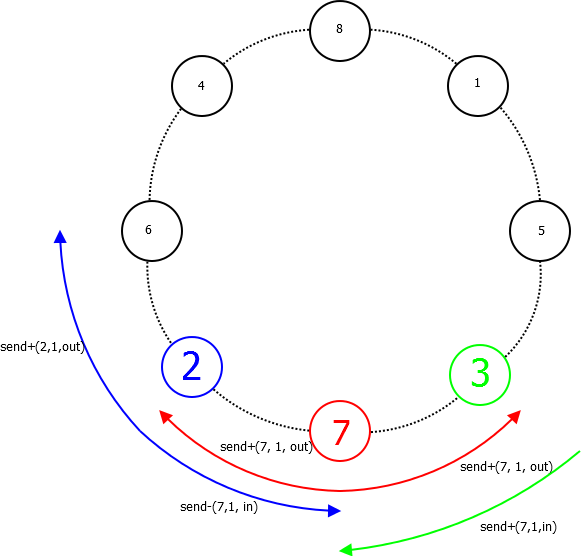
\includegraphics[width=310px]{gfx/HS_p1.png}
	\captionof{figure}{HS Phase 1}
	\label{img:hs_p1}
\end{minipage}

\begin{minipage}{\linewidth}
	\centering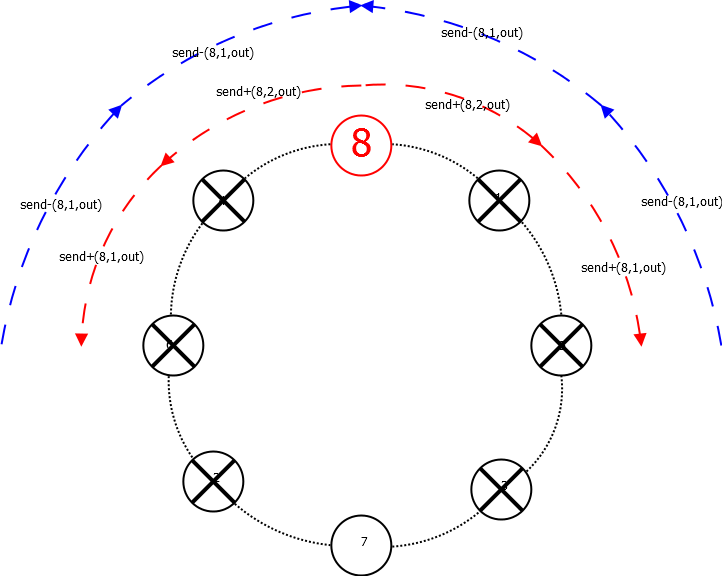
\includegraphics[width=310px]{gfx/HS_p2.png}
	\captionof{figure}{HS Phase 2}
	\label{img:hs_p2}
\end{minipage}

\begin{minipage}{\linewidth}
    \centering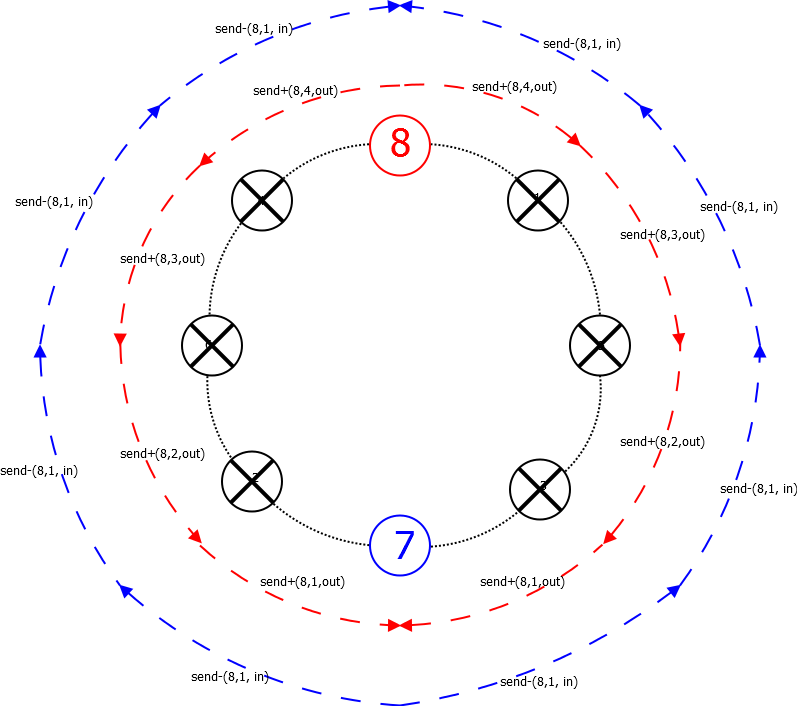
\includegraphics[width=310px]{gfx/HS_p3.png}
    \captionof{figure}{HS Phase 3}
    \label{img:hs_p3}
\end{minipage}

\begin{minipage}{\linewidth}
	\centering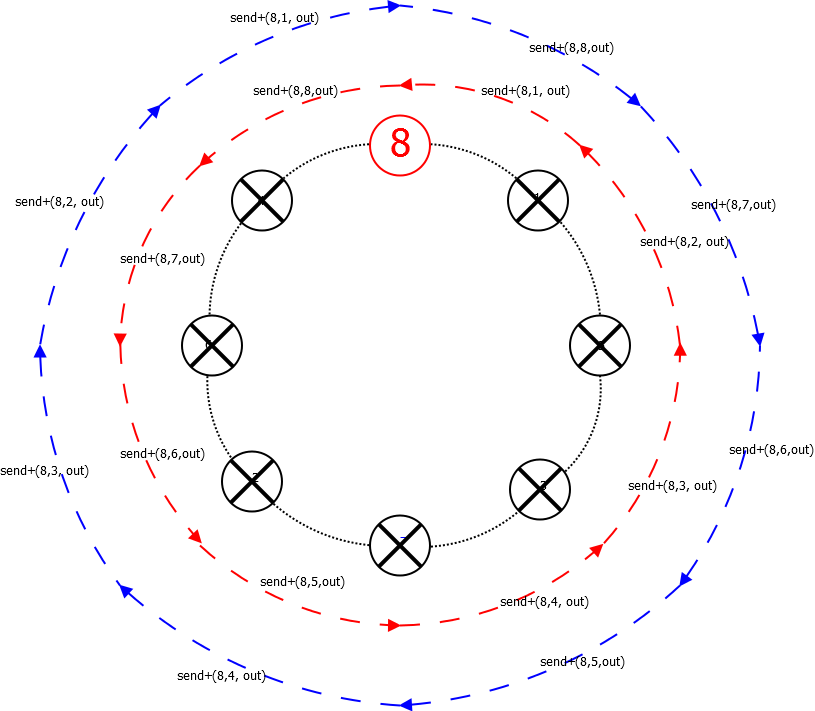
\includegraphics[width=310px]{gfx/HS_p4.png}
	\captionof{figure}{HS Phase 4}
	\label{img:hs_p4}
\end{minipage}

\textbf{Show that the number of messages sent by the HS is at most $8n(1+\left\lceil logn\right\rceil )$, which means it is $O(nlog(n))$.}\\ 
In Phase $k$ können maximal $4\cdot2^{k}$ Nachrichten (in und out) für einen Kandidaten (Knoten, der in seiner Nachbarschaft keinen größeren Knoten hat) existieren.\\
In Phase $k=0$ gibt es $n$ Kandidaten $\Rightarrow$ $2n$ out Nachrichten und maximal $\frac{n}{2}\cdot2$ in Nachrichten $=3n$\\
In Phase $k\geq1$ gibt es maximal noch $\left\lfloor \frac{n}{2^{k-1}+1}\right\rfloor $ Kandidaten. $2^{k-1}+1$ ist der minimale Abstand zwischen zwei Gewinnern aus Phase $k-1$\\ $\Rightarrow$ die Anzahl der Nachrichten, die in Phase $k$ gesendet werden ist $4\cdot2^{k}\cdot\left\lfloor \frac{n}{2^{k-1}+1}\right\rfloor =8n\cdot\left\lfloor \frac{2^{k-1}}{2^{k-1}+1}\right\rfloor $\\ 
Offensichtlich ist die maximale Anzahl der Phasen ist $\left\lceil logn\right\rceil +1$\\
Offensichtlich werden in der letzten Phase $2n$ Nachrichten gesendet\\
$3n+\sum\limits _{k=1}^{\left\lceil logn\right\rceil -1}\left(8n\cdot\left\lfloor \frac{2^{k-1}}{2^{k-1}+1}\right\rfloor \right)+2n\leq5n+8n\cdot\left(\left\lceil logn\right\rceil -1\right)$ 


\subsection{Time slice algorithm}
\begin{compactitem}
	\item ring size $n$ is known
	\item unidirectional
	\item elects smallest UID
	\item Counter-example algorithm: impractical, but useful as lower bound
	\item TimeSlice is much more strongly based on synchronization than LCR
	\begin{compactitem}
		\item The fact that a node did not receive a message in a certain round provides information
	\end{compactitem}
\end{compactitem}


\begin{lstlisting}[mathescape, language=VHDL]
	phases with n rounds
	in phase v consisting of rounds $(v-1) \cdot n+1$,$\dots$,v$\cdot$n only a token carrying UID v is permitted
	if a process with UID v exists and round $(v-1)\cdot n+1$ is reached without having received any messages, then it elects itself the leader and sends a token with it's UID
\end{lstlisting}

\begin{minipage}{\linewidth}
	\centering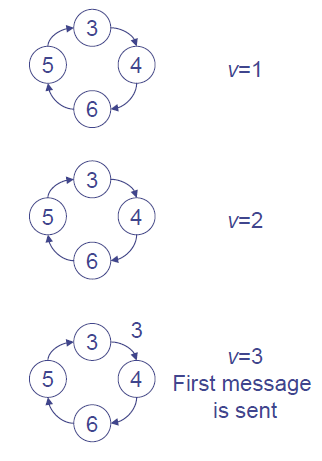
\includegraphics[width=150px]{gfx/timeslice.png}
	\captionof{figure}{Timeslice algorithm}
	\label{img:timeslice}
\end{minipage}


\subsubsection{Complexity}
\begin{compactdesc}
	\item[Communication complexity] number of messages is $\mathcal{O}(n)$
	\item[Time complexity] $n\cdot uid_{min}$
\end{compactdesc}

\subsection{Variable speeds algorithm}

\subsubsection*{Algorithm}
\begin{compactitem}
\item each process $i$ creates a token to travel around the ring, carrying UID u of origin
\item tokens travel at differrent speed
\item token carrying UID v travels  1 messages every $2^{v}$ rounds (slow down)
\item each process memorises smallest UID
\item return to origin elects UID (smallest UID is selected as leader)
\end{compactitem}

\subsubsection*{Complexity}

\begin{compactdesc}
	\item[Communication complexity] $\sum\limits_{k=1}^n \frac{1}{2^{k-1}} (<2n) \Rightarrow \mathcal{O}(n)$
	\item[Time complexity] $n\cdot uid_{min}$ (i.e. slow)
\end{compactdesc}

\section{Leader election in a wireless environment}
\begin{compactitem}
\item consider time needed for communication
\item every node can initiate an election
\item the select is based on information like battery lifetime or processing power (that is the value sent back in step 7/8)
\item the nodes only participate in one election, also there are more than one initiating nodes
\end{compactitem}

\subsubsection*{Algorithm}
\begin{compactenum}
\item one node starts the election and sends ELECT to its neighbours
\item the node, which sended the ELECT message becomes the parent of the node
\item the node sends the request to all neighbours except the parent node
\item the node acknowledges the parent after all the children acknowledged the election
\item if a node recieves an ELECT message, but has already a parent, it responses immediately, that another node is its parent (i.e. an ack without a value)
\item if a the node has only neighbours, which are the parent or have other parents, the node becomes a leaf and sends back its value
\item the waiting nodes send the node id and the max value of the children (or himself) to the parent, after all acknowledged
\item in the end, the initiating node knows the node with the highest value and broadcast to all nodes, that this is the leader
\end{compactenum}

\begin{minipage}{\linewidth}
	\centering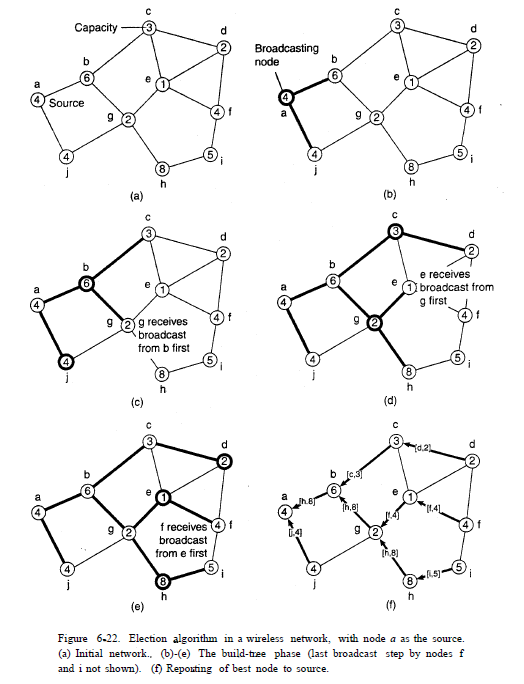
\includegraphics[width=310px]{gfx/Leader_adhoc.png}
	\captionof{figure}{Election in wireless networks}
	\label{img:Leader_adhoc}
\end{minipage}

\section{The Bully Algorithm(flooding) (Garcia-Mdina, 1982)}
- process P holds election
\begin{compactenum}
\item P sends ELECT message to all processes with higher uid
\item P wins if there are no responses $\Rightarrow$ P is leader and sends COORDINATOR message to all available nodes.
\item if Q (with higher uid) answers with OK, Q takes over and sends ELECT to all higher nodes again.
\end{compactenum}

\begin{minipage}{\linewidth}
	\centering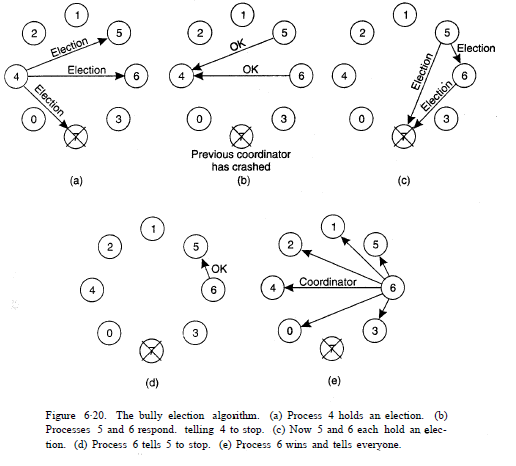
\includegraphics[width=310px]{gfx/leader1.png}
	\captionof{figure}{The bully election algorithm}
	\label{img:leader1}
\end{minipage}

